\chapter{Дослідження криптографічних протоколів системи PayPal}

\section{Загальні теоретичні основи побудови платіжних систем}
Платіжні системи є комплексними структурами, що забезпечують електронний обмін фінансовими даними між учасниками. Вони відіграють ключову роль у сучасній економіці, забезпечуючи швидкість, зручність і безпеку фінансових транзакцій. Основні аспекти, що визначають платіжні системи:


\begin{itemize}

    \item \textbf{Криптографічний захист.} Криптографія є основою безпеки платіжних систем. Вона забезпечує три ключові властивості, які є необхідними для захисту фінансових транзакцій та конфіденційності даних користувачів.
    
    \item \textbf{Конфіденційність.} Конфіденційність у платіжних системах досягається шляхом шифрування даних, що передаються між учасниками. Алгоритми шифрування, такі як AES (Advanced Encryption Standard), забезпечують високий рівень захисту інформації. Вони використовують симетричний підхід, де один і той самий ключ застосовується як для шифрування, так і для розшифрування даних. Важливим аспектом конфіденційності є динамічне генерування ключів, яке ускладнює їх компрометацію. Наприклад, при використанні протоколу TLS (Transport Layer Security), сесійний ключ генерується для кожного з'єднання, що мінімізує ризики перехоплення. Також застосовується захист від атак на основі аналізу трафіку. Це дозволяє приховати не тільки самі дані, але й метадані, такі як розмір транзакцій чи IP-адреси учасників. Таким чином, конфіденційність забезпечує не тільки приватність даних, але й захист від можливих дій зловмисників.
    \item \textbf{Цілісність.} Цілісність даних гарантується через використання криптографічних хеш-функцій, таких як SHA-256 (Secure Hash Algorithm). Ці функції генерують унікальний "відбиток" для кожного блоку даних, що дозволяє виявити будь-які зміни, навіть мінімальні. У платіжних системах хеш-функції застосовуються для перевірки транзакцій: отримувач може порівняти хеш отриманих даних із хешем, надісланим відправником. Якщо значення збігаються, дані вважаються цілісними. Додатково застосовуються механізми MAC (Message Authentication Code), які об'єднують хеш-функції та секретні ключі. Це дозволяє захистити дані від підробки навіть у разі перехоплення їх зловмисником. Цілісність є критично важливою для запобігання зміні суми транзакції або реквізитів отримувача.
    \item \textbf{Аутентифікація.} Аутентифікація забезпечує підтвердження особи учасників транзакції. Одним із найпоширеніших методів є використання цифрових сертифікатів, які видаються центрами сертифікації (CA). Цифровий сертифікат містить унікальні дані користувача та його відкритий ключ, що дозволяє перевіряти підписані повідомлення. Електронні підписи, створені за допомогою алгоритмів, таких як RSA або ECDSA, гарантують, що повідомлення надіслано дійсним користувачем і не було змінено під час передачі. У платіжних системах також широко використовується двофакторна аутентифікація, яка включає пароль і додатковий фактор, наприклад, одноразовий код або біометричні дані (відбиток пальця чи розпізнавання обличчя).

\end{itemize}

Таким чином, криптографічний захист є багатошаровим процесом, який охоплює конфіденційність, цілісність та аутентифікацію, створюючи надійний фундамент для безпеки платіжних систем.

\section{Про протокол SET}


Secure Electronic Transactions (SET) був розроблений компаніями Visa та Mastercard у 1996 році для забезпечення безпеки електронних платежів через Інтернет. Основною метою SET є захист конфіденційності платіжних даних, автентифікація всіх учасників транзакції та забезпечення цілісності переданої інформації. 

\begin{figure}[ht]
        \centering
        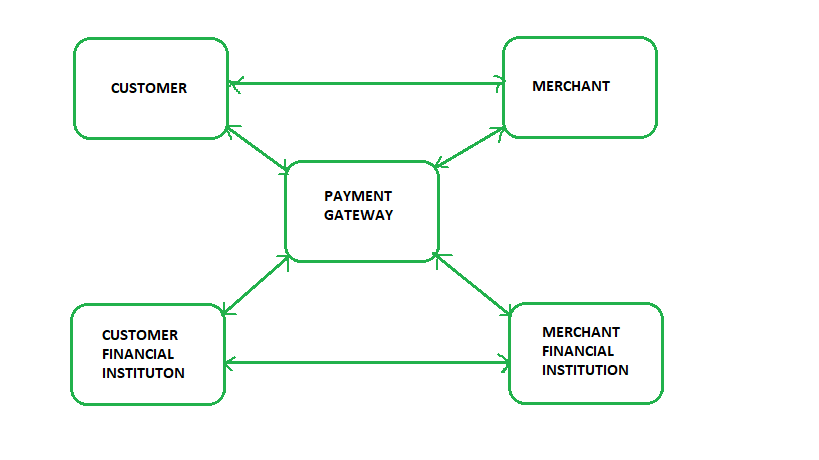
\includegraphics[scale=0.8]{../IMAGES/transaction-scenario.png}
        \label{transaction-scenario}
    \end{figure}


Завдяки використанню криптографічних методів, таких як цифрові сертифікати, електронні підписи та шифрування, SET значно знижує ризики шахрайства та атак на платіжні системи.

\subsection{Учасники протоколу SET}

\begin{itemize}
    \item \textbf{Клієнт (покупець)}: Клієнт є ініціатором транзакції та використовує свою банківську картку для здійснення платежу. Для автентифікації клієнт використовує сертифікат цифрового підпису, який підтверджує його особу. При цьому конфіденційність інформації про картку забезпечується завдяки шифруванню, яке виконується ще на стороні клієнта перед передачею даних. Таким чином, продавець не має доступу до фінансової інформації клієнта.

    \item \textbf{Продавець}: Продавець відповідає за приймання замовлення та ініціацію платіжного процесу. Через використання протоколу SET продавець також має сертифікат, який підтверджує його легітимність. Це виключає можливість здійснення фіктивних транзакцій. Продавець надсилає запит на оплату через платіжний шлюз, не маючи доступу до чутливої інформації клієнта, оскільки дані про картку шифруються.

    \item \textbf{Банк-емітент}: Банк-емітент є організацією, яка видала клієнту банківську картку. Його функція в протоколі SET полягає у перевірці автентичності клієнта, доступності коштів на рахунку та авторизації транзакції. Банк отримує запит на підтвердження через платіжний шлюз і обробляє його з дотриманням усіх криптографічних вимог SET.

    \item \textbf{Платіжний шлюз}: Це посередник між продавцем та банком, який забезпечує безпечну передачу платіжної інформації. Шлюз здійснює дешифрування даних та передає їх банку-емітенту для перевірки. Також він забезпечує зворотний зв'язок між банком та продавцем, інформуючи про результат обробки транзакції. Платіжний шлюз працює за принципом ``чорного ящика'', не зберігаючи жодної чутливої інформації.
\end{itemize}

\subsection{Функції протоколу SET}

Протокол Secure Electronic Transactions (SET) створений для забезпечення високого рівня безпеки електронних платежів через Інтернет. Він об'єднує кілька ключових функцій, кожна з яких спрямована на захист даних, автентифікацію учасників і збереження цілісності транзакцій. Ось детальний розгляд його основних функцій:


\begin{figure}[ht]
        \centering
        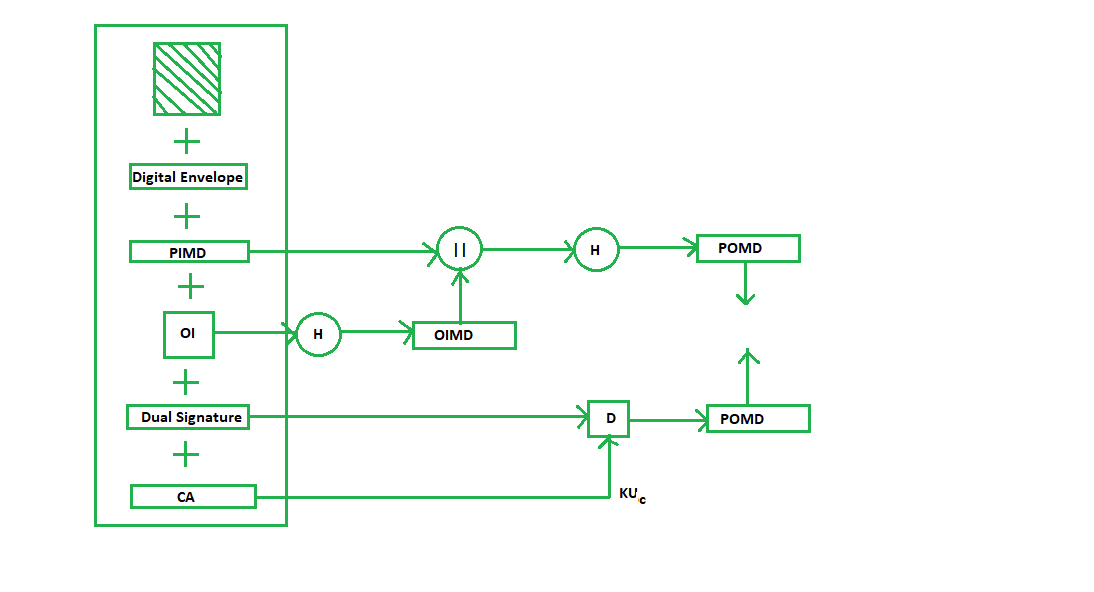
\includegraphics[scale=0.8]{../IMAGES/Purchase-Request-Validation.png}
        \label{prval}
    \end{figure}

\begin{itemize}
    \item \textbf{Шифрування даних}: Шифрування є фундаментальною функцією SET, яка забезпечує конфіденційність інформації, що передається між учасниками. Для цього SET використовує симетричні алгоритми, такі як DES (Data Encryption Standard), для шифрування чутливих даних, включаючи номери банківських карток, суми платежів та іншу фінансову інформацію. Перевага симетричного шифрування полягає в його високій швидкості обробки великих обсягів даних. Однак для передачі ключів між учасниками SET використовує асиметричне шифрування (наприклад, RSA), що гарантує безпеку процесу обміну ключами. Таким чином, SET поєднує переваги обох методів шифрування, забезпечуючи ефективний та надійний захист.

    \item \textbf{Цифрові сертифікати}: Одним із найбільших ризиків у сфері електронних платежів є підробка учасників транзакцій. Для вирішення цієї проблеми SET використовує цифрові сертифікати формату X.509, які видаються сертифікаційними центрами (Certificate Authorities, CA). Ці сертифікати містять зашифровану інформацію про власника, включаючи його ім'я, публічний ключ і підпис центру сертифікації. Верифікація автентичності відбувається на всіх етапах транзакції. Клієнт підтверджує свою особу продавцю, продавець підтверджує свою легітимність клієнту, а платіжний шлюз та банк забезпечують взаємну довіру між фінансовими установами. Такий багаторівневий процес гарантує, що транзакція виконується лише між авторизованими сторонами.

    \item \textbf{Аутентифікація та авторизація}: SET забезпечує двосторонню аутентифікацію, де кожна сторона підтверджує свою особу. Авторизація платежу виконується банком-емітентом після підтвердження автентичності клієнта та продавця. Це зменшує ризик фальсифікації платежів.

    \item \textbf{Цілісність даних}: Цілісність даних є критично важливим аспектом безпеки електронних платежів. Протокол SET використовує криптографічні хеш-функції, такі як SHA-1 або MD5 (на момент створення SET), для генерування унікальних хешів повідомлень. Ці хеші додаються до повідомлень перед їх передачею і перевіряються одержувачем. Якщо навіть один біт даних зміниться під час передачі, згенерований хеш більше не збігатиметься з початковим, що сигналізує про порушення цілісності. Такий підхід дозволяє оперативно виявляти будь-які спроби модифікації даних, включаючи атаки "людина посередині".
\end{itemize}

Таким чином, протокол SET забезпечує комплексний підхід до захисту електронних платежів, зменшуючи ризики шахрайства та несанкціонованого доступу. Завдяки своїй криптографічній основі SET став прототипом для багатьох сучасних платіжних систем.

Хоча SET сьогодні рідко використовується через складність реалізації та низьку продуктивність у сучасних масштабах, його функції стали основою для багатьох сучасних протоколів. Наприклад, принципи шифрування, автентифікації та забезпечення цілісності, реалізовані в SET, є основними компонентами таких технологій, як TLS (Transport Layer Security) та сучасних платіжних систем, наприклад, Visa Secure та Mastercard SecureCode.

\section{Безпека системи електронних платежів PayPal}

PayPal є однією з найпоширеніших платформ для здійснення електронних платежів, і її популярність значною мірою обумовлена надійною системою безпеки. Платформа забезпечує швидкі, зручні та безпечні розрахунки, об'єднуючи мільйони користувачів у глобальну мережу електронної комерції. Одна з основних переваг PayPal — багаторівневий підхід до захисту даних, що включає передові технології та інноваційні алгоритми.

\subsection{Двофакторна аутентифікація}

Одним із ключових механізмів безпеки PayPal є двофакторна аутентифікація (2FA). Ця система вимагає підтвердження особи користувача за допомогою двох незалежних компонентів: паролю (щось, що знає користувач) і коду, отриманого через SMS, мобільний додаток або апаратний токен (щось, що є у користувача). 

Цей механізм суттєво знижує ризик несанкціонованого доступу навіть у випадку компрометації паролю. Наприклад, якщо зловмисник отримає пароль, без другого фактору аутентифікації він не зможе увійти до облікового запису. Додатково, PayPal використовує систему моніторингу пристроїв та IP-адрес. Якщо виявляється спроба входу з нового пристрою або підозрілої локації, користувача можуть попросити пройти додаткову перевірку.

\subsection{Токенізація}

Токенізація є ще одним важливим елементом безпеки PayPal. Цей процес передбачає заміну конфіденційних даних користувача, таких як номер кредитної картки або банківського рахунку, на унікальні токени, які не мають жодного сенсу для сторонніх осіб. 

Наприклад, під час транзакції PayPal не передає продавцю реальні дані картки покупця, а замість цього використовує токен. Такий підхід суттєво зменшує ризик компрометації даних навіть у випадку злому бази даних продавця. Якщо зловмисник отримає токен, він не зможе використати його для виконання інших транзакцій чи отримання інформації про картку.

\subsection{Алгоритми машинного навчання}

Система безпеки PayPal активно використовує алгоритми машинного навчання для виявлення шахрайських транзакцій у реальному часі. Ці алгоритми аналізують велику кількість даних, таких як історія транзакцій, поведінка користувача, геолокація та інші параметри. 

На основі цього формується профіль звичайної поведінки кожного користувача. Коли транзакція виходить за межі звичного профілю, система може автоматично заблокувати її або позначити як підозрілу для подальшого аналізу. Наприклад, якщо користувач зазвичай здійснює покупки в одній країні, але раптово виконує платіж із зовсім іншої локації, система може зупинити транзакцію до підтвердження її легітимності.

\subsection{Додаткові заходи безпеки}

Окрім основних механізмів, PayPal забезпечує захист через шифрування всіх переданих даних за допомогою SSL/TLS. Це гарантує, що дані не можуть бути перехоплені під час передачі між клієнтом і сервером. 

Також PayPal надає користувачам захист покупця (Buyer Protection), який дозволяє повернути кошти у випадку неотримання товару або отримання товару, що не відповідає опису. Цей механізм не лише сприяє захисту інтересів клієнта, а й підвищує довіру до платформи з боку продавців.

\subsection{Інтеграція PayPal із сторонніми системами}

PayPal також забезпечує високий рівень безпеки під час інтеграції з іншими платформами електронної комерції. Платформа підтримує API для передачі даних між продавцями та клієнтами, використовуючи при цьому найсучасніші протоколи шифрування. 

Продавці отримують доступ до інструментів моніторингу та аналітики, які дозволяють відслідковувати підозрілу активність і своєчасно реагувати на потенційні загрози.

\subsection{Захист від фішингових атак}

PayPal активно бореться з фішинговими атаками, інформуючи користувачів про способи розпізнавання підроблених листів або вебсайтів. Усі офіційні повідомлення від PayPal містять імена користувачів, що допомагає відрізнити їх від фальшивих.

Також компанія впроваджує системи виявлення та блокування фішингових доменів, співпрацюючи з міжнародними організаціями з кібербезпеки.

\section{Висновок до розділу 3}

Завдяки багаторівневій системі захисту, використанню токенізації, алгоритмів машинного навчання та двофакторної аутентифікації, PayPal забезпечує надійну платформу для електронних платежів. Безпека, прозорість і захист інтересів клієнтів залишаються головними пріоритетами компанії, що робить її одним із лідерів у сфері електронної комерції.
